\documentclass{standalone}
%
\usepackage{tikz}
\usepackage{pgfplots}
\pgfplotsset{width=10cm,compat=1.9}

\usepackage{xcolor}
\definecolor{space}{HTML}{0A2543}
%
\title{The Witch of Agnesi}
\begin{document}
	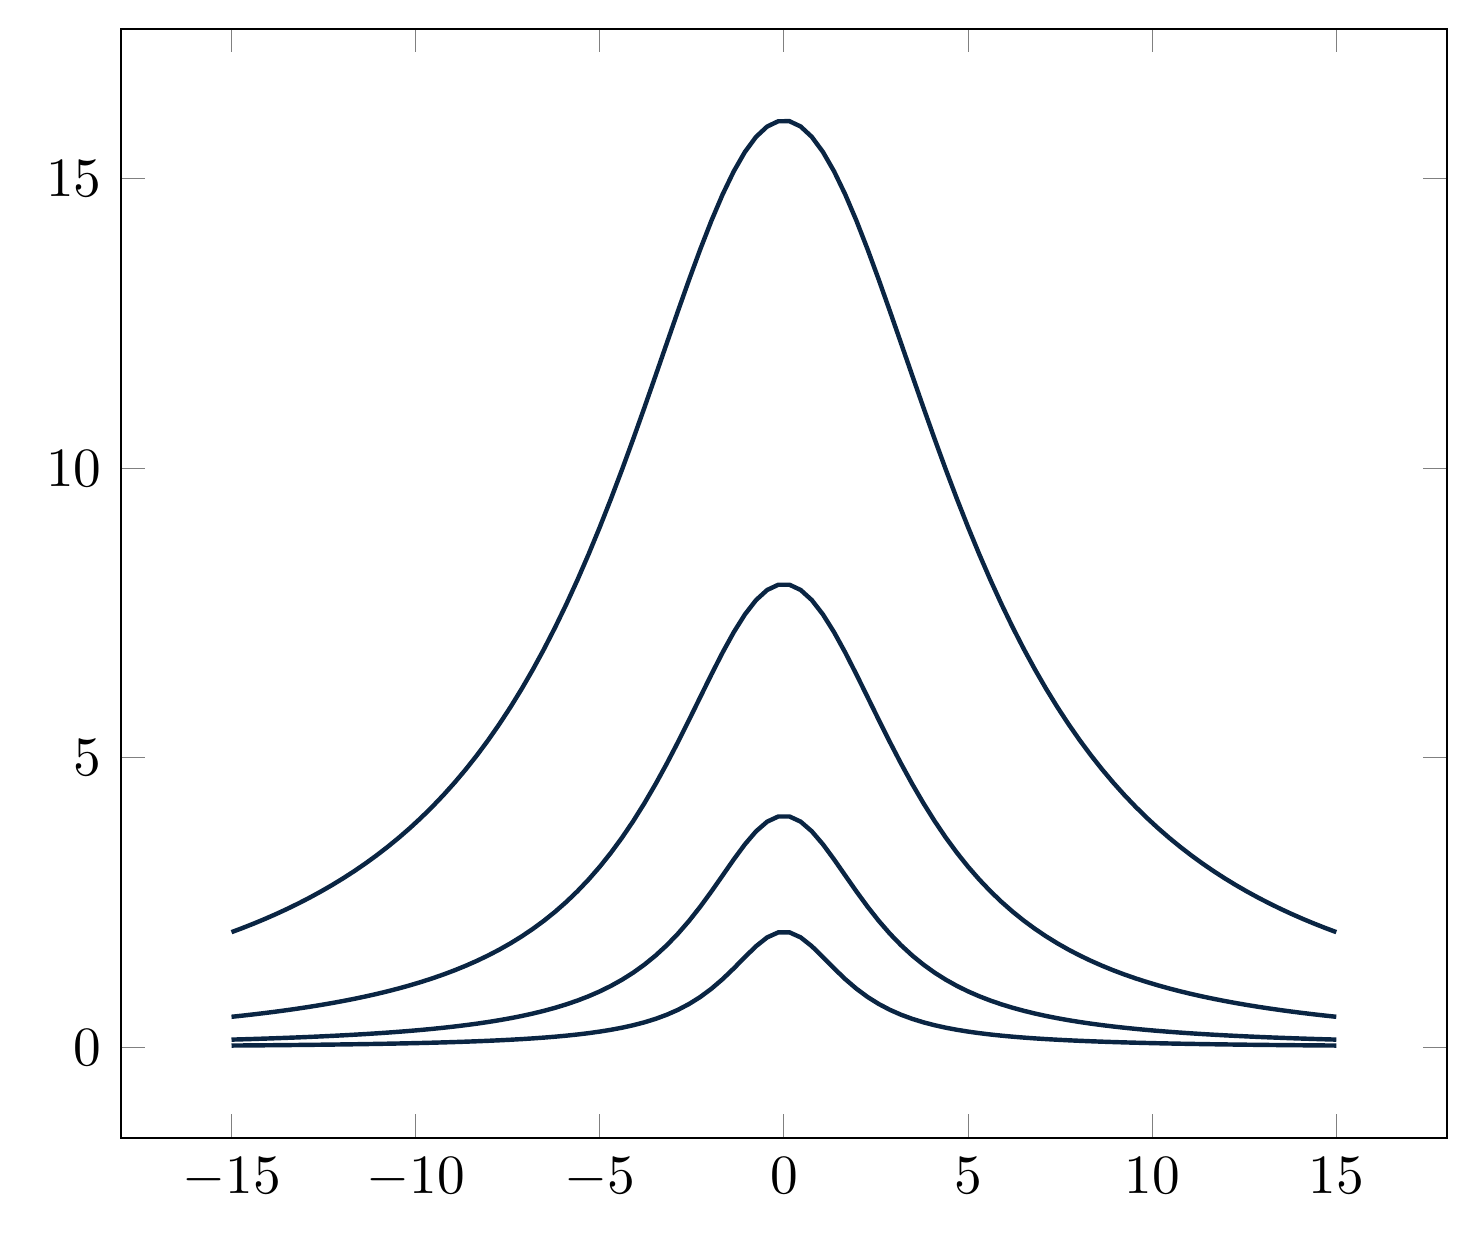
\begin{tikzpicture}[domain=-15:15]
		\begin{scope}[scale=2]
			\begin{axis}
				\foreach \a in {1,2,4,8}
					\addplot [domain=-15:15, samples=100, color=space, thick]{8 * \a^2 / (x^2 + 4 * \a)};
			\end{axis}
		\end{scope}
	\end{tikzpicture}
\end{document}